\documentclass[fontset=windows, 12pt]{article}
\usepackage[a4paper, total={6.5in, 10in}]{geometry}
\usepackage{ctex}
\usepackage{wasysym}
\usepackage{graphicx}
\usepackage{float}
\usepackage{tikz}
\usepackage{manfnt}
\usepackage{calligra}

\newcommand{\trans}[1]{\songti 翻译注释:#1}

\title{Book Printing versus Ordinary Typing}
\author{Eureka}
\date{\today}
\begin{document}
\maketitle
    
\section{引号}

单引号的背景:

American keyboards usually contain a left-quote
character that shows up as something like \`, and an apostrophe or right-quote
that looks like ' or ´.

使用样例: `single-quote'


\bigskip
双引号的背景:

To produce double-quote marks with TEX, you simply type two single-
quote marks of the appropriate kind.

使用样例: ``double-quote''


\section{\TeX 中用到的字符}
Here are the symbols to be used (you might type on your terminal):

\begin{verbatim}
        ABCDEFGHIJKLMNOPQRSTUVWXYZ
        abcdefghijklmnopqrstuvwxyz
        0123456789"#$%&@*+-=,.:;?!
        ()<>[]{}‘’\|/_^~
\end{verbatim}

\textbf{Remark}

If your computer terminal doesn't happen to have all of these, don’t despair;
TEX can make do with the ones you have

\trans{make do with-凑合着用}

\clearpage
\section{不同的 -}
    dashes\hspace*{10em}
    hyphens:(着重符号)

    minus signs:(减号)\hspace*{10em}
    En-dash:()

    Em-dash:()\hspace*{10em}
    bibliography:()

    ligatures:()\hspace*{10em}
    kerning:()

    \begin{figure}[!htb]
        \centering  
        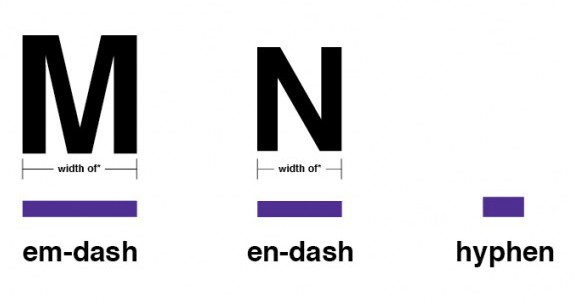
\includegraphics[scale=0.5]{./Pic/dash.jpg}
        \label{dash}
        \caption{dashes}
        \verb |图片来源:https://zhuanlan.zhihu.com/p/54652480|
    \end{figure}

\textbf{Basic Four Usage}
\begin{enumerate}
    \item Hyphens are used for compound words like ‘daughter-in-law’ and ‘X-rated’.
    \item En-dashes are used for number ranges like `pages 13--34'
    \item Em-dashes are used for punctuation in sentences---they are
    what we often call {\bf simply dashe}s.
    \item minus signs are used in formulas, $1-1=0$.
\end{enumerate}


\textbf{How To Type These Four item}
\begin{enumerate}
    \item for a hyphen, type a hyphen (-);
    \item for an en-dash, type two hyphens (--);
    \item for an em-dash, type three hyphens (---);
    \item for a minus sign, type a hyphen in mathematics mode ($-$).
\end{enumerate}

记忆方法:M 比 N 要大,所以 em-dash 要多一个 -


\section{ligatures(连字)}
If you look closely at most well-printed books, you will find that certain
combinations of letters are treated as a unit.

For example, this is true of the {\bf `f'} and the {\bf `i'} of {\bf `find'}.

常见的连字:{\bf ff, fi, fl, ffi, ffl}

使用连字的原因:The reason is that words like {\bf `f\/ind'} don't look
very good in most styles of type unless a ligature is substituted for the letters
that clash. 

\textbf{Remark:取消连字}\\
1. 推荐:\verb |f\/ind| --> {\bf f\/ind}\\
2. \verb |Di{f}{f}erent| --> {\bf Di{f}{f}erent}\\
3. 使用bable宏包加上 ngerman 选项\\
详情参考:\verb |https://tex.stackexchange.com/questions/439651/how-do-i-disable-ligatures|

\section{EXERCISE}
$\RHD$  EXERCISE 2.1

Explain how to type the following sentence to TEX: Alice said, ``I always use an
en-dash instead of a hyphen when specifying page numbers like `480--491' in a
bibliography.''

\bigskip

\textbf{Solve}\\
{The Above Code Is the Answer}






$\RHD$  EXERCISE 2.2

What do you think happens when you type four hyphens in a row?


\bigskip
\textbf{Solve}\\
1. type \verb |Hello----world| in this row: Hello----world

$\RHD$  EXERCISE 2.3 

Think of an English word that contains two ligatures ?

\textbf{Solve}\\
The good news is that you do not have to concern yourself with liga-
tures: TEX is perfectly capable of handling such things by itself, using the same
mechanism that converts `\verb |--|' into `--'. In fact, TEX will also look for combi-
nations of adjacent letters (like `A' next to `V' ) that ought to be moved closer
together for better appearance; this is called {\bf kerning}.

\trans{kerning:字距调整}

\trans{翻译:你不必担心, \TeX 内部会自动处理  ... 类似. \TeX 也会自动调整adjacent(形状)的两个字母(比如A和V)的间距 ...}

\textbf{Remark: An Exmaple of kerning}\\
{A}V~~(不用 kerning 处理)\\
AV~~(使用后)
\begin{tikzpicture}[overlay,remember picture]
    \draw[red] (-5.4em, 2.5em)--(-5.4em, -1em);
\end{tikzpicture}

放大之后你参考那一条红色的辅助线,就可以轻松的看出 kerning 的作用了。


\section{Summary}

总结:这一章主要讲了以下的几点:\\
1. 你应该怎么 \textbf{抄代码} --- quote 和 hyphen 的问题\\
2. 你该怎么输入代码 --- ligature 和 kerning 的问题


\section{Enhance}
\lhdbend  继续前面的讨论,如果你键盘上面真的没有左右引号怎么办 ?

\bigskip
{\bf 原文参考}

If your keyboard does not contain a left-quote symbol, {\bf you can type \verb |\lq|,
followed by a space if the next character is a letter, or followed by a \textbackslash{} if the
next character is a space.} Similarly, \verb |\rq| yields a right-quote character.


一个应用举例:\verb |\lq Hello\rq\ World| ---> \lq Hello\rq\ World

注: 如果不添加最后的 \textbackslash\ 的话,那么结果就是:\lq Hello\rq World


\begin{figure}[!htb]
    \centering
    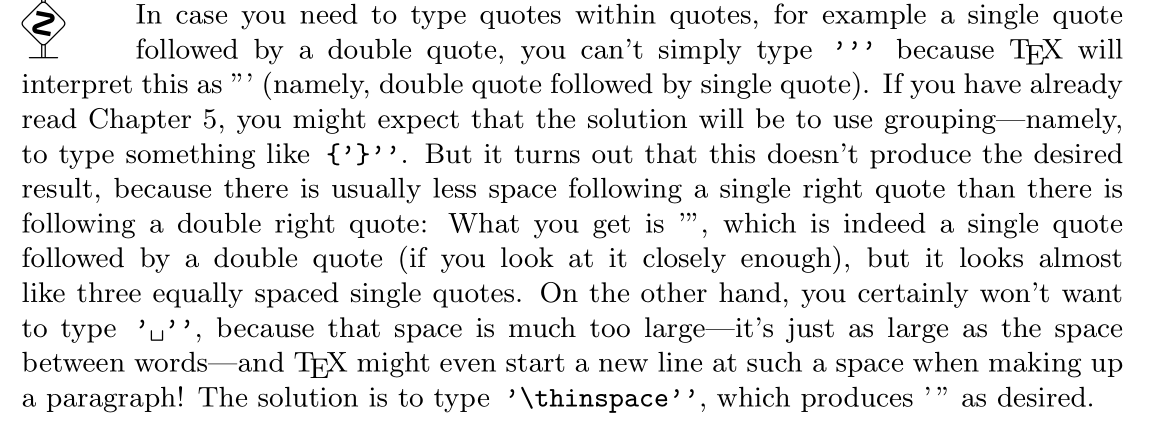
\includegraphics[scale=0.65]{./Pic/quote.png}
    \label{quote}
\end{figure}


\vspace*{10em}
\centering
\calligra{The End}

\end{document}